\documentclass{article}

\usepackage{graphicx}
\usepackage{tikz}
\usepackage{tikzsymbols}
\usetikzlibrary{calc,patterns,shapes.geometric}
\pagestyle{empty}
\usepackage[margin=0pt]{geometry}
\geometry{papersize={14in,12in}}

\def\centerarc[#1](#2)(#3:#4:#5){\draw[#1] ($(#2)+({#5*cos(#3)},{#5*sin(#3)})$) arc (#3:#4:#5);}

\begin{document}
	\begin{figure}
		\centering
		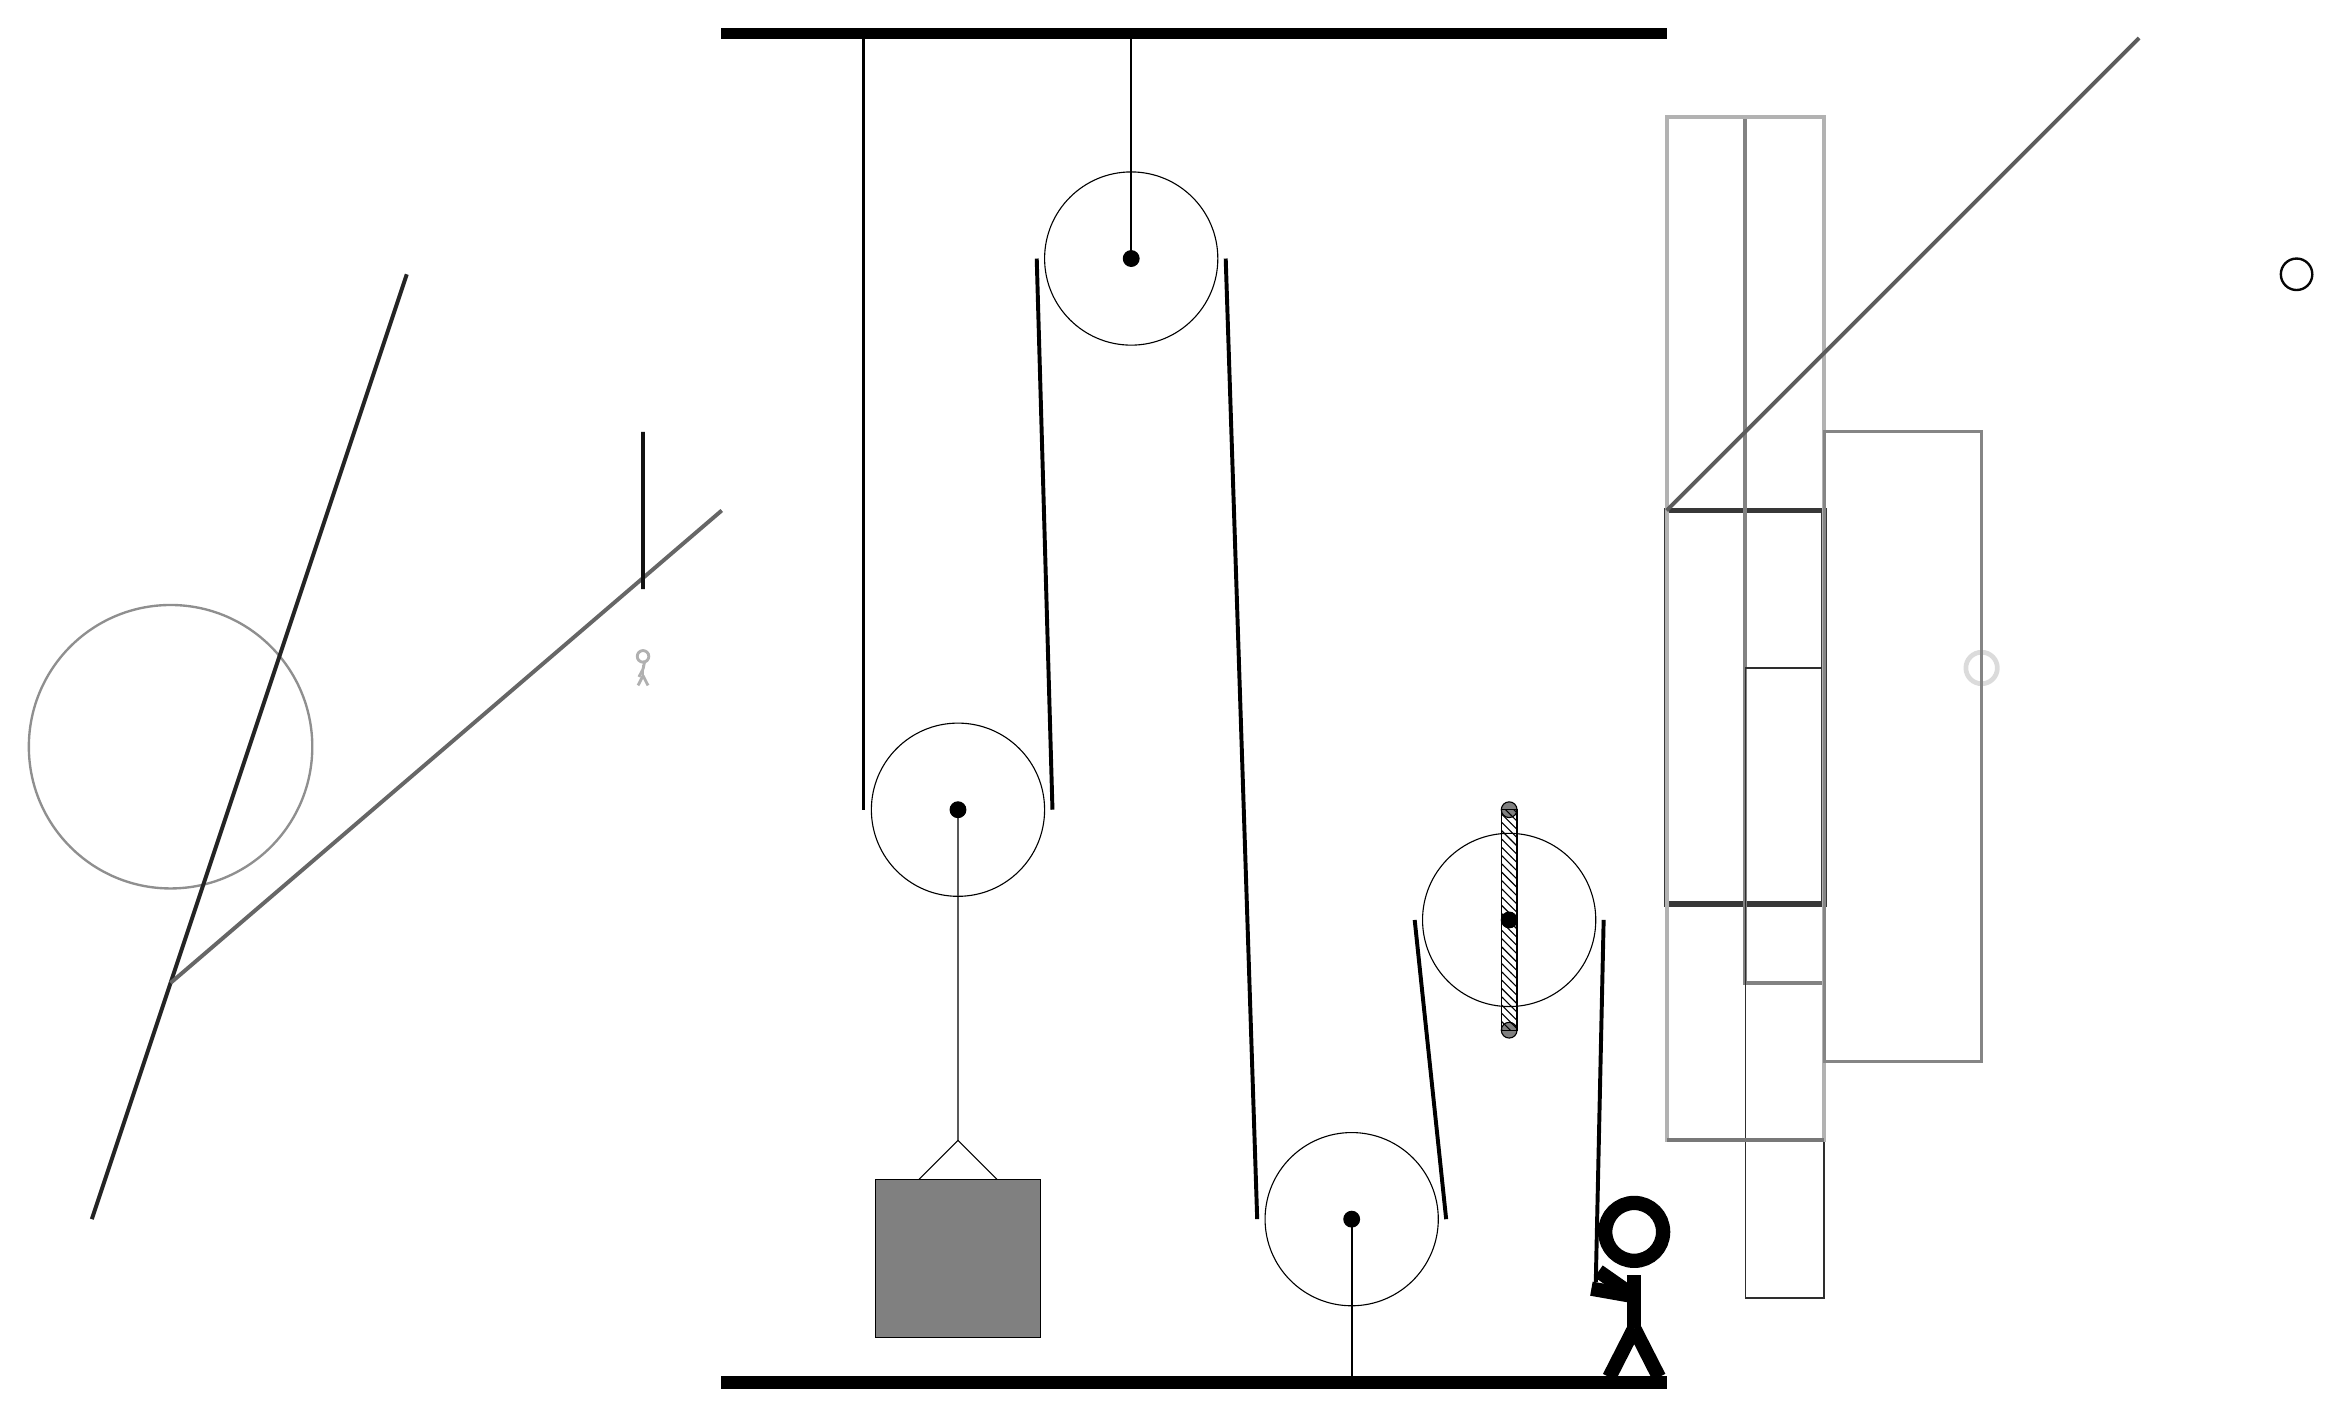
\begin{tikzpicture}
			%%%%% START %%%%%
			
			\draw[fill=black] (-2, 14) rectangle (10, 14.125);
			
			\draw (1, 4.2) circle (1.1);
			\draw[fill=black] (1, 4.2) circle (0.1);
			
			\draw (3.2, 11.2) circle (1.1);
			\draw[fill=black] (3.2, 11.2) circle (0.1);
			\draw[thick] (3.2, 11.2) -- (3.2, 14);
			
			\draw (6, -1) circle (1.1);
			\draw[fill=black] (6, -1) circle (0.1);
			\draw[thick] (6, -1) -- (6, -3);
			
			\draw[fill=white](8, 2.8) circle (1.1);
			\draw[fill=black] (8, 2.8) circle (0.1);
			\draw[fill=black!50] (8, 4.2) circle (0.1);
			\draw[fill=black!50] (8, 1.4) circle (0.1);
			\draw[pattern=north west lines, pattern color=black] (7.9, 4.2) rectangle (8.1, 1.4);
			
			\draw (1, 4.2) -- (1, 0) -- (0.5, -0.5);
			\draw (1, 0) -- (1.5, -0.5);
			\draw[fill=black!50] (-0.05, -0.5) rectangle (2.05, -2.5);
			
			\draw [line width=0.3mm, color=black!44](-9, 5) circle (1.8);
			
			\draw[line width=0.7mm, color=black!78] (10, 3) rectangle (12, 8);
			\draw[line width=0.5mm, color=black!49] (11, 2) rectangle (12, 13);
			\draw[line width=0.2mm, color=black!82] (11, -2) rectangle (12, 6);
			\draw [line width=0.6mm, color=black!14](14, 6) circle (0.2);
			\node[line width=0.5mm, color=black!31] at (-3, 6) {\Strichmaxerl[2][62][78]};
			
			\draw[line width=0.5mm, color=black!86](-6, 11) -- (-10, -1);
			\draw[line width=0.5mm, color=black!30] (10, 13) rectangle (12, 0);
			\draw[line width=0.4mm, color=black!48] (12, 9) rectangle (14, 1);
			\draw[line width=0.5mm, color=black!60](-2, 8) -- (-9, 2);
			
			\draw[line width=0.5mm, color=black!93] (-3, 9) rectangle (-3, 7);
			\draw[line width=0.5mm, color=black!53](12, 0) -- (10, 0);
			\draw [line width=0.3mm, color=black!98](18, 11) circle (0.2);
			\draw[line width=0.5mm, color=black!64](10, 8) -- (16, 14);
			
			\draw[line width=0.5mm] (-0.2, 14) -- (-0.2, 4.2);
			\centerarc[line width=0.5mm](1, 4.2)(180:360:1.2000000000000002);
			\draw[line width=0.5mm](2.2, 4.2) -- (2.0, 11.2);
			\centerarc[line width=0.5mm](3.2, 11.2)(0:180:1.2000000000000002);
			\draw[line width=0.5mm](4.4, 11.2) -- (4.8, -1);
			\centerarc[line width=0.5mm](6, -1)(180:360:1.2000000000000002);
			\draw[line width=0.5mm](7.2, -1) -- (6.8, 2.8);
			\centerarc[line width=0.5mm](8, 2.8)(0:180:1.2000000000000002);
			\draw[line width=0.5mm](9.2, 2.8) -- (9.1, -1.8);
			
			\node at (9.5, -1.9) {\Strichmaxerl[10][-35][170]};
			
			\draw[fill=black] (-2, -3) rectangle (10, -3.15);
			
			%%%%% END %%%%%
		\end{tikzpicture}
	\end{figure}	
\end{document}